\documentclass[a4paper,11pt]{article}
\usepackage[top=3cm, bottom=3cm, left = 2cm, right = 2cm]{geometry} 
\usepackage[utf8]{inputenc}
\usepackage[portuguese]{babel}
\usepackage{graphicx} 
\usepackage{amsmath,amssymb}  
\usepackage{tabularx}
\usepackage{fancyhdr}
\usepackage{enumitem}
\usepackage{hyperref}
\usepackage{ragged2e}
\usepackage[dvipsnames]{xcolor}
\usepackage{bm}  
\usepackage{minted}
\usepackage{textcomp}
\usepackage{import}
\usepackage{memhfixc} 
\usepackage{pdfsync}  
\usepackage{booktabs}

\graphicspath{ {../assets/} }

\pagestyle{fancy}
\fancyhead[L]{}

\parindent 0px

\title{Relatório da Atividade 1}
\author{Aluno: Victor Jorge Carvalho Chaves \\ RA: 156.740}
\date{Data: 24/03/2024}

\begin{document}

\maketitle

\section{Estudo dos Dados}

Na base de dados do Titanic, há várias colunas que podem ser interessantes ou não para serem aplicadas no treinamento de uma Árvore de Decisão. Visto isso, é importante o entendimento da natureza desses dados e a validação de usá-los para o teste ou não.

\subsection{Análise das Colunas}

\begin{itemize}[label=--]
    \item Survived: É o valor que é necessário ser previsto
    \item Pclass: Representa qual a classe social, podendo ser relevante na sobrevivência do indivíduo
    \item Name: Nome do indivíduo, a princípio, não deve ser relevante na previsão
    \item Sex: Sexo do indivíduo, por questões culturais, pode ter afetado na taxa de sobrevivência
    \item Age: Idade do indivíduo, por questões culturais, pode ter afetado na taxa de sobrevivência
    \item SibSp: Quantidade de parentes, pode ser relevante na previsão
    \item Parch: Quantidade de filhos ou pais, pode ser relevante na previsão
    \item Ticket: Ticket do passageiro, não aparenta ser necessário
    \item Fare: Taxa de pagamento, a princípio, não aparenta ser relevante
    \item Cabin: A posição de sua cabine pode ser importante, porém há muitos dados faltando
    \item Embarked: Representa a origem de embarcação no Titanic
    \item PassengerId: Id de referência do passageiro, não é relevante para a análise
\end{itemize}

\pagebreak

\section{Descrição das Variáveis da Árvore de Decisão}
\subsection{Profundidade Máxima (\texttt{max\_depth})}

Determina a altura máxima que a árvore de decisão pode tomar.

\subsection{Critério (\texttt{criterion})}
O critério é um parâmetro que determina a medida usada para avaliar a qualidade de uma divisão. Em geral, os critérios mais comuns são o Gini e a entropia.

\subsubsection{Gini}
O índice de Gini é uma medida de impureza que avalia quão frequentemente um elemento escolhido aleatoriamente seria classificado incorretamente se fosse classificado aleatoriamente de acordo com a distribuição das classes no nó.

\subsubsection{Entropia}
A entropia é outra medida de impureza que indica o quão "desorganizado" ou "misturado" está um conjunto de dados em relação às classes de destino.

\subsection{Separador (\texttt{splitter})}
O separador define a estratégia usada para escolher a melhor divisão em cada nó da árvore. Os métodos mais comuns são "best" e "random".

\subsubsection{Método ''best''}
Avalia todas as possíveis divisões em um nó e seleciona a melhor delas com base em algum critério de qualidade

\subsubsection{Método ''random''}
A divisão em cada nó será escolhida de forma aleatória entre um subconjunto das melhores divisões possíveis

\subsection{Mínimo de amostras divididas (\texttt{min\_sample\_split})}
O mínimo de amostras divididas é um parâmetro que controla o número mínimo de amostras necessárias para considerar dividir um nó em um nó interno. Se o número de amostras em um nó for menor do que o mínimo de amostras divididas, o nó não será dividido e se tornará uma folha na árvore.

\pagebreak

\section{Análise sobre a variação dos parâmetros}

Considerando o uso das seguintes colunas para o treino:
\begin{itemize}[label=--]
    \item Pclass
    \item Sex
    \item Parch
    \item Fare
    \item Embarked
\end{itemize}

Será realizado vários treinos variando os parâmetros:

\begin{itemize}[label=--]
    \item \texttt{max\_depth}: Sem limite, 2 e 4
    \item \texttt{criterion}: "gini" e "entropy"
    \item \texttt{splitter}: "best" e "random"
    \item \texttt{min\_sample\_split}: 2 e 10
\end{itemize}

E considerando o resultado dos seguintes testes...

\begin{table}[htbp]
    \centering
    \caption{Resultados dos experimentos}
    \label{tab:resultados}
    \begin{tabular}{ccccccc}
        \toprule
        balanced accuracy  & max\_depth & splitter & criterion & min\_sample\_split \\
        \midrule
        1.0                & 2          & random   & entropy   & 10                 \\
        1.0                & 2          & random   & gini      & 2                  \\
        1.0                & 2          & random   & gini      & 10                 \\
        0.8651315789473684 & 4          & best     & entropy   & 2                  \\
        0.8651315789473684 & 4          & best     & entropy   & 10                 \\
        0.8463345864661653 & 4          & best     & gini      & 2                  \\
        0.8463345864661653 & 4          & best     & gini      & 10                 \\
        0.806860902255639  & None       & best     & entropy   & 10                 \\
        0.7922932330827068 & None       & best     & gini      & 10                 \\
        0.7838345864661653 & None       & best     & entropy   & 2                  \\
        0.763157894736842  & 2          & best     & entropy   & 2                  \\
        0.763157894736842  & 2          & best     & entropy   & 10                 \\
        0.763157894736842  & 2          & best     & gini      & 2                  \\
        0.763157894736842  & 2          & best     & gini      & 10                 \\
        0.7579887218045113 & 4          & random   & entropy   & 2                  \\
        0.7579887218045113 & 4          & random   & entropy   & 10                 \\
        0.7579887218045113 & 4          & random   & gini      & 2                  \\
        0.7579887218045113 & 4          & random   & gini      & 10                 \\
        0.7532894736842106 & None       & random   & entropy   & 10                 \\
        0.7387218045112782 & None       & random   & gini      & 10                 \\
        0.7194548872180451 & None       & best     & gini      & 2                  \\
        0.7175751879699248 & None       & random   & entropy   & 2                  \\
        0.7109962406015038 & None       & random   & gini      & 2                  \\
        \bottomrule
    \end{tabular}
\end{table}

\subsection{Variação do Critério (\texttt{criterion})}

É notável que o método de Entropia e Gini variam bem por toda a amostra de testes, não se dividem bem entre a melhor acurácia e a pior.

Isso deve ser causado por conta que o dado do Sexo é o primeiro a ser usado na árvore de decisão, e divide a maioria dos casos de morte.

Na image abaixo é possível ver o formato da árvore de decisão quando a altura máxima é 1.

\begin{figure}[h]
    \centering
    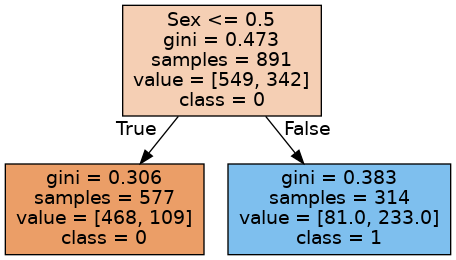
\includegraphics[width=0.5\textwidth]{sex.png}
    \caption{Árvore de decisão criada com altura máxima como 1}
    \label{fig:nome_para_referenciar}
\end{figure}

A partir disso, notamos que o sexo é a classe que divide a maior parte.

E considerando o gráfico abaixo


\begin{figure}[h]
    \centering
    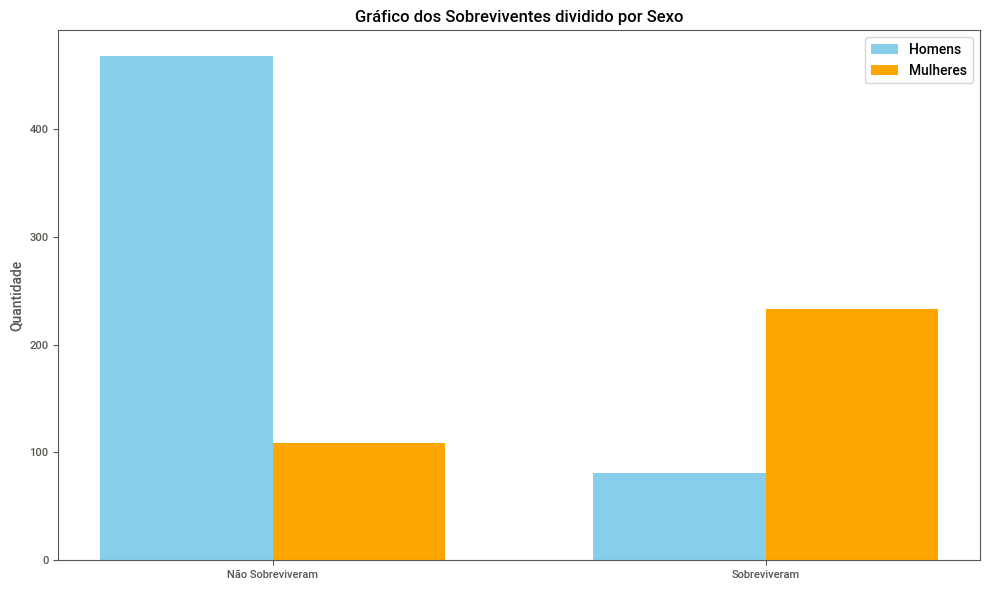
\includegraphics[width=1\textwidth]{output.png}
    \caption{Gráfico dos Sobreviventes dividido por Sexo nos dados de treino}
    \label{fig:nome_para_referenciar}
\end{figure}

Notamos que a maioria dos sobreviventes foram as mulheres, e a maioria dos homens que morreram, por volta 19\% dos homens sobreviveram, e 75\% das mulheres sobreviveram.

Com esse tipo de divisão que separa já 68\% dos sobreviventes e 76\% dos que não sobreviveram, fica difícil com esse estados dos dados de ver uma diferença relevante do uso do Gini e da Entropia, já que independente qual seja usado, ambos chegam na conclusão que o Sexo é a melhor categoria a ser usada. Usando ela primeiro, já é possível alcançar ótimos resultados, tendo assim o aperfeiçoamento dependente de outros fatores...

Porém em contexto que usam a mesma profundidade e método de divisão, entropia tem mostrado resultados relativamente melhores.

\subsection{Variação Separador (\texttt{splitter})}

Em uma combinação do uso do método random e uma profundidade máxima de 2, é alcançando o melhor resultado de 100\%.

É interessante que uma profundidade baixa alcança bons resultados usando o método random, nesse contexto, categorias que de forma aleatória apresentam menor chance de erro se beneficiaram nesse contexto com poucas decisões. Enquanto com uma árvore de profundidade maior apresentou o pior dos resultados.

Enquanto isso, o método best alcança abaixo do random os melhores resultados, sendo os melhores aqueles que usam de uma profundidade de 4 com o critério de entropia.

\subsection{Variação do \texttt{min\_sample\_split}}

Não apresentou grande diferenças na acurácia balanceada, talvez com valores maiores poderia ver diferença nos resultados.


\subsection{Variação do \texttt{max\_graph}}

A profundidade vária na acurácia dependendo principalmente da combinação do uso do método de divisão, e por segundo, o critério de divisão.

\section{Árvore de decisão Escolhida}

A partir desses dados, a melhor árvore de decisão a ser escolhida é a com seguinte configuração:

\begin{itemize}[label=--]
    \item \texttt{max\_depth}: 2
    \item \texttt{criterion}: "entropy"
    \item \texttt{splitter}: "random"
    \item \texttt{min\_sample\_split}: 10
\end{itemize}

O motivo dessa escolha é por conseguir alcançar a melhor acurácia no teste de 100\%, ter o método de entropia, que apresenta uma pequena melhora nos resultados comparado ao gini, um método de divisão "random" que permite alcançar os 100\% com uma árvore de tamanho máximo 2.

Porém é necessário considerar que os dados de teste são tendenciosos, já que constam que 100\% das mulheres sobreviveram e 100\% dos homens morreram, assim possibilitando o alcance dos 100\% de acurácia.

\end{document}
